\documentclass[twocolumn]{article}
\usepackage{graphicx}
\usepackage{titling}

\title{Optimización de Arbitraje de BESS mediante Pronóstico del Costo Marginal de Generación en el Sistema Eléctrico Chileno}
\author{Gonzalo Iglesias, Nicolás Sotelo, Max Cruz  \\
    Pontificia Universidad Católica de Chile  \\
    }
\date{\today}

\usepackage{polyglossia}
\setdefaultlanguage{spanish}

% Define the path for images
\graphicspath{{./articulo/imgs/}}

\begin{document}

\maketitle

\begin{abstract}
El precio de venta de la energía (Costo Marginal o CMg) en el mercado spot chileno se determina por el costo de la unidad más cara despachada en el sub-sistema respectivo. Para optimizar la rentabilidad de BESS que retiran e inyectan al sistema mediante el mercado spot es crucial tener una estimación de los costos en el corto plazo (24-48 horas). Este trabajo realiza un análisis de rendimiento de tres arquitecturas avanzadas de deep learning para el pronóstico del CMg: una Red Neuronal Convolucional de Grafos (GCN) combinada con GRU, un Transformer para series temporales (Informer) y un modelo híbrido Transformer + CNN (TFT) para capturar patrones estacionales y relaciones de largo alcance. El proyecto busca identificar la arquitectura más precisa para apoyar la toma de decisiones en el almacenamiento energético, optimizando el arbitraje.
\end{abstract}

\section{Introducción}
Durante la última década, Chile ha experimentado un rápido crecimiento en la penetración de energías renovables no convencionales (ERNC) en la zona norte, lo que no ha sido acompañado por un aumento equivalente en la capacidad de transmisión. Esto ha causado congestiones en la transmisión, lo cual afecta el Costo Marginal de Generación (CMg) al generar precios bajos o nulos en las zonas con sobreoferta. Para maximizar la rentabilidad de BESS, es crucial identificar patrones en la variabilidad del CMg en el corto plazo (24-48 horas). En este proyecto se evaluarán tres arquitecturas de deep learning con el objetivo de comparar su efectividad en la predicción de CMg y contribuir al conocimiento científico mediante el análisis de su capacidad para capturar patrones de largo y corto alcance en series temporales energéticas.

\section{Metodología}
\subsection{Datos}
Para el entrenamiento de los modelos, se utilizarán datos históricos:
\begin{itemize}
    \item \textbf{Demanda Nacional}: demanda eléctrica en MW, desde 2018 con resolución horaria.
    \item \textbf{Disponibilidad de ERNC}: pronóstico de ERNC en MW por central, por hora.
    \item \textbf{Matriz de Generación}: potencia instalada por tecnología en MW desde 2018.
    \item \textbf{Cotas de Embalse}: niveles de embalse de las principales centrales hidroeléctricas.
\end{itemize}

\subsection{Modelos}
Para abordar el problema, evaluamos tres arquitecturas de deep learning con capacidades para capturar relaciones espaciotemporales en el CMg.
\begin{enumerate}
    \item \textbf{GCN + GRU}: combina una GCN para modelar la red de transmisión, capturando interacciones espaciales, con una capa GRU para dependencias temporales.
    \item \textbf{Informer}: un Transformer optimizado para series largas, ideal para detectar patrones de largo alcance en la demanda y disponibilidad energética.
    \item \textbf{TFT (Transformer + CNN)}: utiliza CNN para estacionalidades de corto plazo y atención para relaciones de largo plazo, adaptándose a la variabilidad del CMg en contextos de alta congestión.
\end{enumerate}

\begin{figure}[htbp]
    \centering
    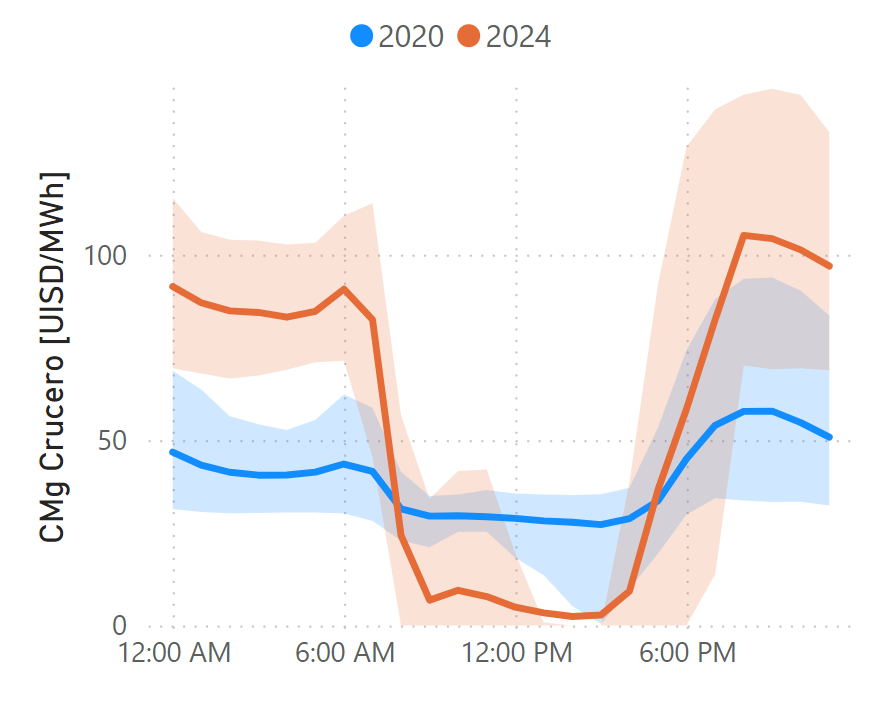
\includegraphics[width=1\columnwidth]{cmg_comparacion.png}
    \caption{Comparación perfil diario CMg promedio pre y post escenario de congestión en barra Crucero 220kV}
    \label{fig:comp_cmg}
\end{figure}

\begin{figure}[htbp]
    \centering
    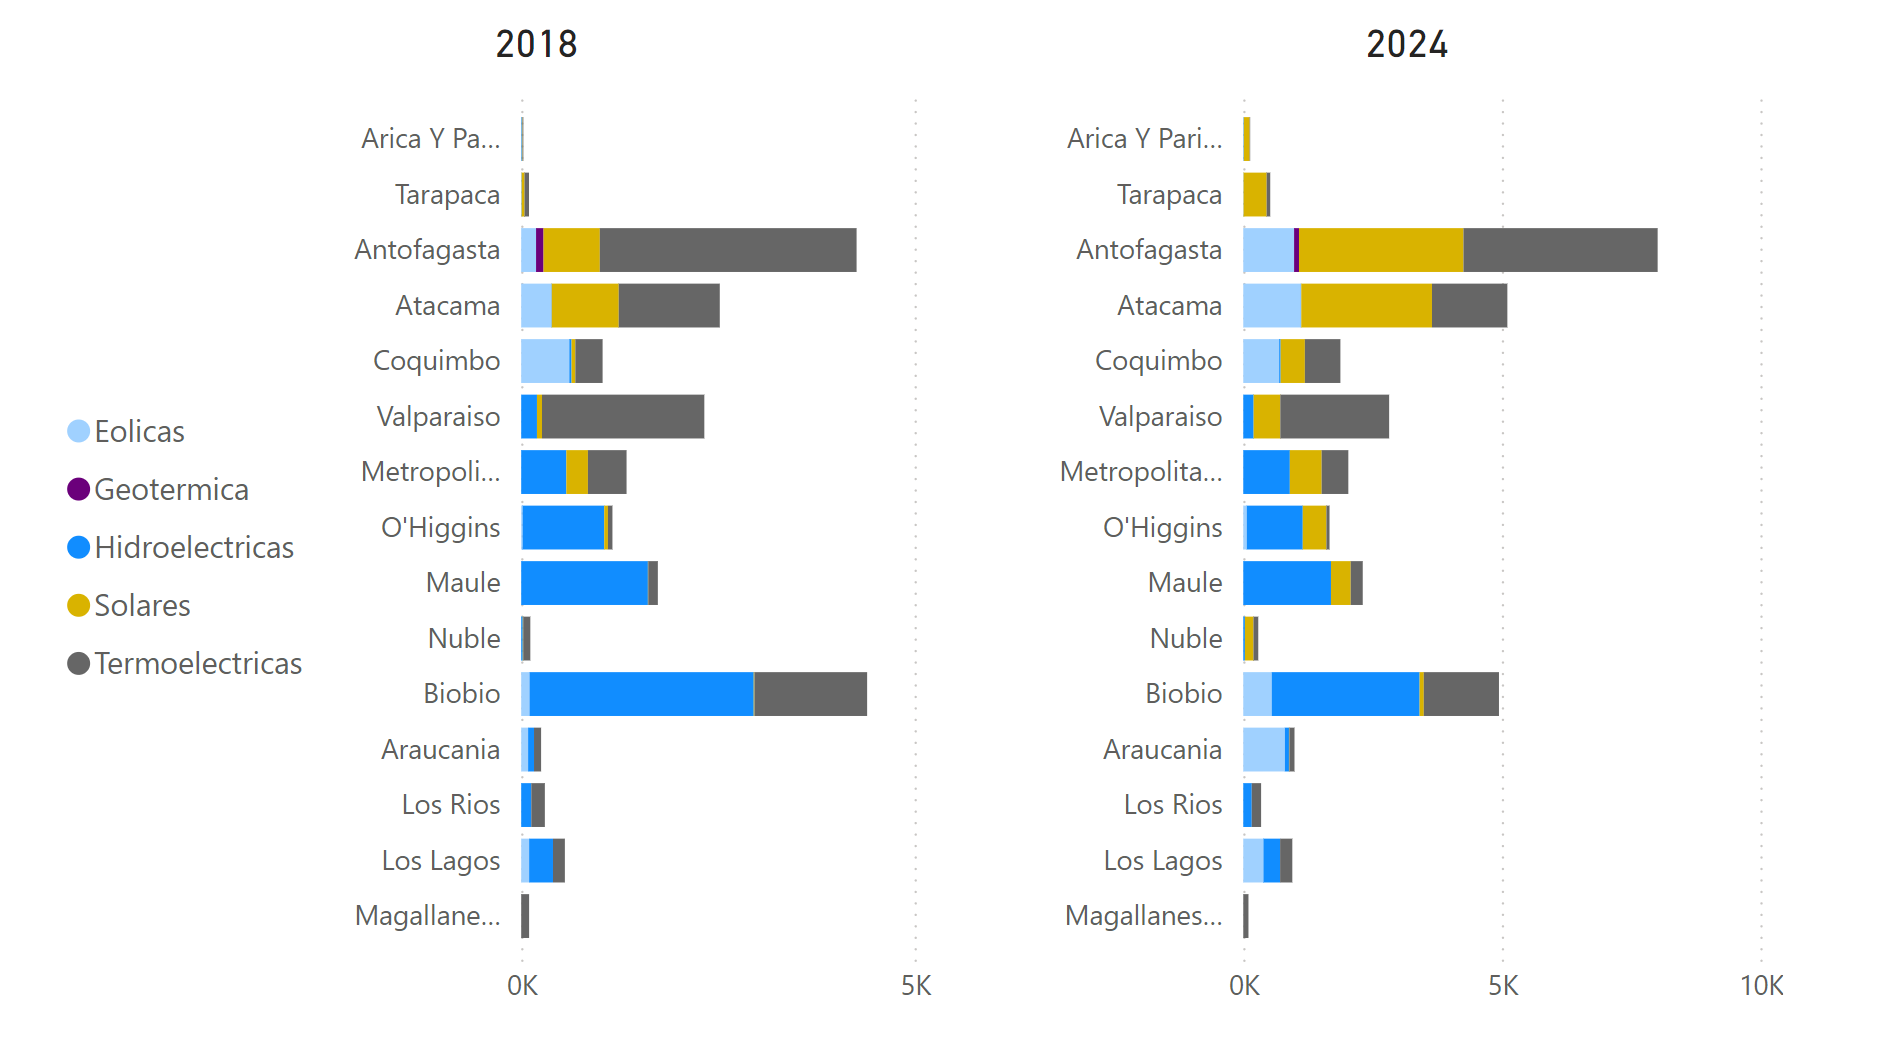
\includegraphics[width=1\columnwidth]{matriz_sist.png}
    \caption{Cambio en la Matriz de Generación del SEN}
    \label{fig:matriz_sistema}
\end{figure}

\section{Conclusión}
Este proyecto proporciona un enfoque comparativo para la predicción del CMg en el sistema energético chileno, utilizando arquitecturas avanzadas de deep learning. A través del análisis del rendimiento de GCN + GRU, Informer y TFT, esperamos identificar la arquitectura que mejor capte la complejidad espaciotemporal del CMg, optimizando el arbitraje en BESS y aportando un nuevo enfoque para el manejo de la volatilidad en sistemas energéticos.

\end{document}
